\documentclass[11pt,a4paper]{ctexart}
\usepackage{geometry}
\geometry{left=2.3cm,right=2.3cm,top=2.2cm,bottom=2.4cm}
\usepackage{amsmath,amssymb,bm}
\usepackage{booktabs}
\usepackage{array}
\usepackage{xcolor}
\usepackage{hyperref}
\usepackage{enumitem}
\usepackage{tcolorbox}
\usepackage{tikz}
\usetikzlibrary{arrows.meta,positioning,fit,shapes.geometric,calc}

\hypersetup{
    colorlinks=true,
    linkcolor=blue!60!black,
    urlcolor=blue!60!black,
    citecolor=blue!60!black
}

\definecolor{deepblue}{RGB}{24,64,120}
\definecolor{teal}{RGB}{0,120,120}
\definecolor{orange}{RGB}{210,90,20}
\definecolor{purple}{RGB}{105,65,150}
\definecolor{softblue}{RGB}{235,245,255}
\definecolor{softorange}{RGB}{255,246,235}
\definecolor{softpurple}{RGB}{245,240,255}
\definecolor{softteal}{RGB}{235,250,248}

\setlist[itemize]{leftmargin=2em}
\setlist[enumerate]{leftmargin=2em}

\title{非线性 local-global latent system、Koopman modal signatures\\与两个 LFP--BOLD 课题的统一框架}
\author{Framework note}
\date{2026-06-10}

\begin{document}
\maketitle

\begin{tcolorbox}[colback=softblue,colframe=deepblue,title=核心观点]
LFP、local BOLD、global BOLD 不应被简单看作 feed-forward input-output 关系，而应看作一个 local-global nonlinear latent system 的不同观测读出。Koopman eigenfunctions 将这个复杂非线性系统转化为可解释的 modal variables，使 global gating state、pre-activation modes、global ROI map 和 loop backbone 成为可操作的 phenomenological modal signatures。
\end{tcolorbox}

\tableofcontents
\newpage

\section{总体图景}

这份笔记总结当前对两个相关课题的统一数学理解：
\begin{enumerate}
    \item \textbf{Event-related LFP subprocess $\to$ global BOLD pattern / BOLD eigenfunction residual}：局部 LFP subprocess 如何作为 intrinsic perturbation，触发或预测全局 BOLD modal innovation。
    \item \textbf{Non-causal LFP--BOLD IR / pre-activation}：为什么 local BOLD 相对于 local LFP 会出现 apparent pre-activation，以及如何用 closed-loop local-global latent dynamics 和 Koopman modal representation 解释。
\end{enumerate}

两个课题对应闭环的两半：
\[
\underbrace{u_{\mathrm{LFP}} \rightarrow x^{(g)}}_{\text{local-to-global: BOLD modal innovation}}
\qquad\text{and}\qquad
\underbrace{x^{(g)} \rightarrow u_{\mathrm{LFP}}}_{\text{global-to-local: pre-activation / gating}}.
\]

合起来，它们描述：
\[
x^{(g)} \rightarrow u_{\mathrm{LFP}} \rightarrow x^{(g)},
\]
即 global order-parameter-like state gates local hippocampal subprocess, and local subprocesses in turn perturb/update global BOLD network state。

\section{最底层模型：分块的非线性 local-global latent system}

令 latent state 分为 local 和 global 两部分：
\begin{equation}
    x_t =
    \begin{bmatrix}
    x_t^{(l)} \\
    x_t^{(g)}
    \end{bmatrix}.
\end{equation}

其中：
\begin{itemize}
    \item $x_t^{(l)}$：local latent state，例如 hippocampal local neural state、local vascular state、local circuit excitability；
    \item $x_t^{(g)}$：global latent state / internal environment / global order-parameter-like state，例如 global brain state、neuromodulatory state、brainstem-thalamic-cortical state、global vascular/arousal state；
    \item $u_t$：local LFP subprocess / local neural action。
\end{itemize}

一个 generic nonlinear model 可以写成：
\begin{align}
    x_{t+1}^{(l)} &= F_l\!\left(x_t^{(l)}, x_t^{(g)}, u_t\right), \\
    x_{t+1}^{(g)} &= F_g\!\left(x_t^{(g)}, x_t^{(l)}, u_t\right),
\end{align}
或简写为：
\begin{equation}
    x_{t+1}=F(x_t,u_t).
\end{equation}

这个模型的关键不是假设 LFP 是外部刺激，而是把 $u_t$ 视为 local subsystem 的 action-like subprocess。它可以暂时作为 input-like variable 写入模型，但在 closed-loop 视角下，它本身也是系统内部生成的。

\section{BOLD 是 nonlinear readout，不是机制本身}

local BOLD 和 global BOLD 都是 latent state 的观测读出：
\begin{align}
    y_t^{(lB)} &= h_l\!\left(x_t^{(l)}, x_t^{(g)}\right), \\
    y_t^{(gB)} &= h_g\!\left(x_t^{(l)}, x_t^{(g)}\right).
\end{align}

因此，local BOLD 不是单纯由 local LFP 经过 HRF 产生的 output。它可以同时包含：
\begin{equation}
    y_t^{(lB)} = \text{local component} + \text{global component}.
\end{equation}

这点非常关键：如果 local BOLD 提前读出了某个 global latent state，那么 local BOLD 相对于未来的 local LFP subprocess 就可能出现 apparent pre-activation。

\section{Global-to-local 路径：global state gates local LFP subprocess}

当前对 pre-activation 的最核心解释是：
\begin{equation}
    x_t^{(g)} \rightarrow u_{\mathrm{LFP},t+\Delta}.
\end{equation}

更具体地，可以写成：
\begin{equation}
    x_t^{(g)} \rightarrow x_{t+\Delta}^{(l)} \rightarrow u_{\mathrm{LFP},t+\Delta}.
\end{equation}

意思是：一个 global latent state / order-parameter-like variable 先出现，然后调节 local hippocampal condition，使某个 local LFP subprocess 更容易发生。

如果要构成完整 closed loop，还可以有 local-to-global 的反向一段：
\begin{equation}
    u_{\mathrm{LFP},t} \rightarrow x_{t+\Delta}^{(g)}.
\end{equation}

因此整体闭环可以概括为：
\begin{equation}
    x^{(g)} \rightarrow u_{\mathrm{LFP}} \rightarrow x^{(g)}.
\end{equation}

但对于 pre-activation 的解释，最关键的是前半段：
\begin{equation}
    x^{(g)} \rightarrow u_{\mathrm{LFP}}.
\end{equation}

\section{为什么 local BOLD--LFP 会产生 apparent non-causal IR？}

传统 feed-forward HRF 模型假设：
\begin{equation}
    y_{\mathrm{localBOLD}}(t)
    =
    \sum_{\tau\ge 0} h(\tau)u_{\mathrm{LFP}}(t-\tau)+\epsilon(t).
\end{equation}

这个模型默认 LFP 是 exogenous input，BOLD 是 passive output。因此，如果 estimated IR 在 $\tau<0$ 有 pre-activation，就看起来像 non-causal。

在 local-global latent model 中，某个 global state $x_t^{(g)}$ 可以同时：
\begin{align}
    x_t^{(g)} &\rightarrow y_t^{(lB)}, \\
    x_t^{(g)} &\rightarrow u_{\mathrm{LFP},t+\Delta}.
\end{align}

于是观测上可能出现：
\begin{equation}
    y_{\mathrm{localBOLD},t}
    \quad \text{早于} \quad
    u_{\mathrm{LFP},t+\Delta}.
\end{equation}

如果这时仍用 feed-forward LFP-to-BOLD deconvolution，就会得到负时滞的 pre-activation。它并不意味着：
\begin{equation}
    y_{\mathrm{localBOLD}} \rightarrow u_{\mathrm{LFP}},
\end{equation}
而是说明：
\begin{equation}
    x^{(g)} \rightarrow
    \begin{cases}
    y_{\mathrm{localBOLD}},\\
    u_{\mathrm{LFP}}.
    \end{cases}
\end{equation}

因此，apparent non-causality 是 closed-loop endogenous system 被 open-loop feed-forward model 误读后的现象。

\section{从非线性系统到增广自治系统}

如果 $u_t$ 是系统内部生成的 local neural action，而不是外部输入，那么可以写作：
\begin{equation}
    u_t = \pi\!\left(x_t^{(g)},x_t^{(l)},u_{t-1},u_{t-2},\ldots\right)+\epsilon_t.
\end{equation}

把 $u_t$ 及其历史增广到状态中：
\begin{equation}
    s_t =
    \begin{bmatrix}
    x_t \\
    u_t \\
    u_{t-1} \\
    \vdots
    \end{bmatrix},
\end{equation}
整个 closed-loop system 可以写成 autonomous form：
\begin{equation}
    s_{t+1}=F_{\mathrm{cl}}(s_t).
\end{equation}

相应的观测读出可写为：
\begin{align}
    u_t &= C_u s_t, \\
    y_t^{(lB)} &= C_l s_t, \\
    y_t^{(gB)} &= C_g s_t.
\end{align}

这一步说明 local LFP subprocess、local BOLD、global BOLD 都可以被看作同一个 autonomous closed-loop system 的不同 readouts。

\section{Koopman modal representation}

对增广自治系统：
\begin{equation}
    s_{t+1}=F_{\mathrm{cl}}(s_t),
\end{equation}
Koopman eigenfunction coordinates 记为 $a_t$，则在 modal coordinate 中：
\begin{equation}
    a_{t+1}=\Lambda a_t.
\end{equation}

观测量可以近似线性读出：
\begin{align}
    u_{\mathrm{LFP},t} &= C_u a_t, \\
    y_{\mathrm{localBOLD},t} &= C_l a_t, \\
    y_{\mathrm{globalBOLD},t} &= C_g a_t.
\end{align}

Koopman 的好处在于：原始 latent dynamics 和 observation functions 都可以是非线性的，但在 lifted/modal space 中，dominant modes、phase relationships 和 spatial readouts 可以被线性或近似线性地分析。

\begin{figure}[ht]
\centering
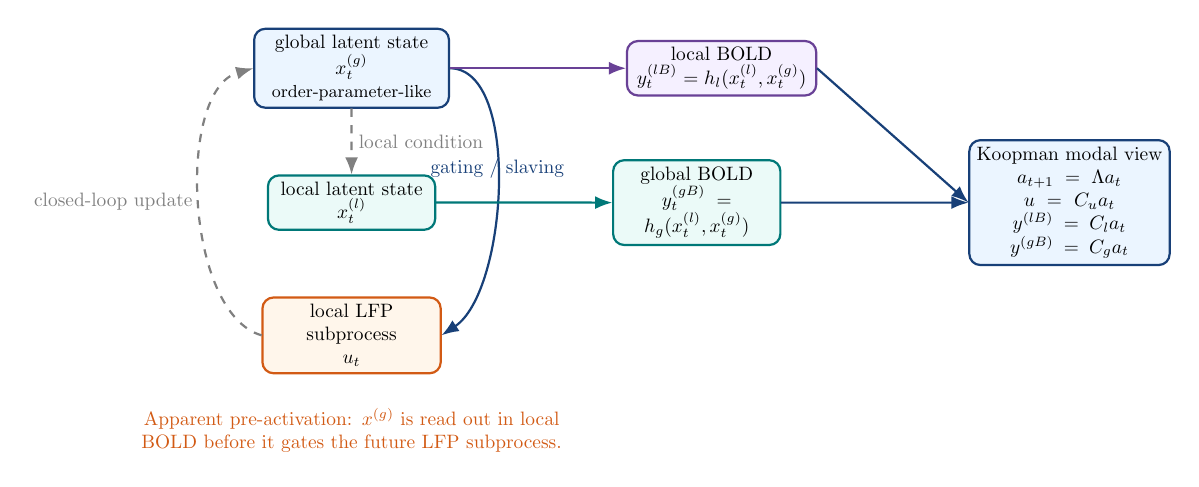
\begin{tikzpicture}[scale=0.70, transform shape,
    node distance=1.4cm,
    box/.style={rounded corners, draw=deepblue, thick, fill=softblue, align=center, minimum height=1.1cm, text width=3.3cm},
    smallbox/.style={rounded corners, draw=teal, thick, fill=softteal, align=center, minimum height=0.9cm, text width=2.8cm},
    orangebox/.style={rounded corners, draw=orange, thick, fill=softorange, align=center, minimum height=0.9cm, text width=3.0cm},
    purplebox/.style={rounded corners, draw=purple, thick, fill=softpurple, align=center, minimum height=0.9cm, text width=3.2cm},
    arrow/.style={-{Latex[length=2.2mm]}, thick},
    dashedarrow/.style={-{Latex[length=2.2mm]}, thick, dashed, gray}
]

\node[box] (global) {global latent state\\$x_t^{(g)}$\\\small order-parameter-like};
\node[smallbox, below=1.2cm of global] (local) {local latent state\\$x_t^{(l)}$};
\node[orangebox, below=1.2cm of local] (u) {local LFP subprocess\\$u_t$};
\node[purplebox, right=3.2cm of global] (lb) {local BOLD\\$y_t^{(lB)}=h_l(x_t^{(l)},x_t^{(g)})$};
\node[smallbox, right=3.2cm of local] (gb) {global BOLD\\$y_t^{(gB)}=h_g(x_t^{(l)},x_t^{(g)})$};
\node[box, right=3.4cm of gb, text width=3.4cm] (koop) {Koopman modal view\\$a_{t+1}=\Lambda a_t$\\$u=C_u a_t$\\$y^{(lB)}=C_l a_t$\\$y^{(gB)}=C_g a_t$};

\draw[dashedarrow] (global) -- node[right, gray] {local condition} (local);
\draw[arrow, deepblue] (global.east) .. controls +(1.3,0) and +(1.2,0.8) .. node[above, deepblue] {gating / slaving} (u.east);
\draw[dashedarrow] (u.west) .. controls +(-1.4,0.4) and +(-1.4,-0.4) .. node[left, gray] {closed-loop update} (global.west);
\draw[arrow, purple] (global.east) -- (lb.west);
\draw[arrow, teal] (local.east) -- (gb.west);
\draw[arrow, deepblue] (lb.east) -- (koop.west);
\draw[arrow, deepblue] (gb.east) -- (koop.west);

\node[align=center, below=0.5cm of u, text width=9cm, color=orange] {Apparent pre-activation: $x^{(g)}$ is read out in local BOLD before it gates the future LFP subprocess.};
\end{tikzpicture}
\caption{Generic nonlinear local-global latent system and Koopman modal interpretation. The key pre-activation explanation is $x^{(g)}\rightarrow y^{(lB)}$ and $x^{(g)}\rightarrow u_{\mathrm{LFP}}$, not $y^{(lB)}\rightarrow u_{\mathrm{LFP}}$.}
\end{figure}

\section{Pre-activation mode 的定义}

对于某个 LFP--BOLD anchor pair $(p,q)$，其中 $p$ 是某个 local LFP band/subprocess，$q$ 是某个 local BOLD ROI 或 local BOLD readout，如果 empirical cross-kernel $h_{q,p}(\tau)$ 在 $\tau<0$ 出现 pre-activation，则可以在 Koopman modes 中寻找贡献这个 negative-lag component 的 modes。

定义：
\begin{equation}
    \mathcal I_{\mathrm{pre}}(q,p)
    =
    \{i: \text{mode } i \text{ contributes to the negative-lag component of pair }(q,p)\}.
\end{equation}

这些 modes 就是该 anchor pair 的 pre-activation modes。它们的 biological interpretation 是：这些 modes 最自然对应一个 global latent gating state / order-parameter-like variable。这个 global state 先被 BOLD readout 观测到，然后 gate 未来的 local LFP subprocess。

重要边界：pre-activation modes 不是 causal modes，而是 pair-conditioned modal signatures。

\section{Phase lead 的 Koopman 解释}

对某个 mode $i$，假设其 continuous-time eigenvalue 为：
\begin{equation}
    \nu_i=\alpha_i+\mathrm{i}\omega_i.
\end{equation}

在 LFP 和 BOLD readout 上的 complex weights 可写为：
\begin{align}
    C_u(i) &= |C_u(i)|e^{\mathrm{i}\phi_{u,i}}, \\
    C_l(i) &= |C_l(i)|e^{\mathrm{i}\phi_{l,i}}.
\end{align}

如果 local BOLD readout 的 phase 领先 LFP readout，则该 mode 会在 LFP--BOLD cross-kernel 中贡献 apparent pre-activation。对应的相位时间差可写作：
\begin{equation}
    \Delta t_{lB-u,i}
    =
    \frac{\operatorname{wrap}(\phi_{l,i}-\phi_{u,i})}{\omega_i},
\end{equation}
具体符号取决于 phase convention。直观上：
\begin{equation}
    \text{BOLD phase leads LFP phase}
    \quad \Rightarrow \quad
    \text{negative-lag contribution in empirical IR}.
\end{equation}

\section{Global ROI map 的含义}

对某个 anchor pair $(q,p)$ 的 pre-activation modes，global ROI map 可定义为：
\begin{equation}
    M_{q,p}(r)
    =
    \sum_{i\in\mathcal I_{\mathrm{pre}}(q,p)} s_i |C_g(r,i)|,
\end{equation}
其中 $r$ 是 global BOLD ROI，$C_g(r,i)$ 是 mode $i$ 在 ROI $r$ 上的 global BOLD readout weight，$s_i$ 是 mode $i$ 对 pair-specific pre-activation 的贡献强度。

解释：
\begin{quote}
    global ROI map 是 pre-activation modes 在全脑 BOLD ROI 空间中的 spatial footprint。
\end{quote}

在 closed-loop / slaving-principle 解释中，它进一步对应：
\begin{quote}
    gate local LFP subprocess 的 global latent state / order-parameter-like variable 在 BOLD 空间中的可观测足迹。
\end{quote}

它不是“哪些 BOLD ROI 反向驱动 LFP”的 causal map，而是“哪些 ROI 共同表达了这个 global gating state”的 map。

\section{Loop backbone 的含义}

对同一组 pre-activation modes，每个 ROI 的 global BOLD readout 不仅有 amplitude，还有 phase：
\begin{equation}
    C_g(r,i)=|C_g(r,i)|e^{\mathrm{i}\phi_{r,i}}.
\end{equation}

global ROI map 使用 $|C_g(r,i)|$，而 loop backbone 使用 $\phi_{r,i}$。

因此：
\begin{quote}
    global ROI map 描述这个 global state 在哪里表达；loop backbone 描述这个 global state 如何在 ROI 空间中按相位顺序表达。
\end{quote}

可以把每个 mode 的 phase order 转成一个 phase-defined adjacency：
\begin{equation}
    A_i(r_1,r_2)=1
    \quad \text{if ROI } r_1 \text{ phase-leads ROI } r_2
    \quad \text{within mode } i.
\end{equation}

然后对 pre-activation modes 聚合：
\begin{equation}
    A_{q,p}^{\mathrm{backbone}}(r_1,r_2)
    =
    \sum_{i\in\mathcal I_{\mathrm{pre}}(q,p)} s_i A_i(r_1,r_2).
\end{equation}

loop backbone 的解释是：pre-activation modes 所定义的 global gating state，在全脑 ROI 空间中的 phase-ordered expression / phase portrait。它是 candidate biological representation / phenomenological modal signature，不是解剖 feedback loop 本身，也不是 interventional causality。

\section{Haken / slaving principle 的对应关系}

这个框架可以与 Haken 的 slaving principle 对应起来：
\begin{equation}
    \text{distributed brain regions}
    \Rightarrow
    \text{global order parameter}
    \Rightarrow
    \text{local fast subprocess}.
\end{equation}

对应到当前问题：
\begin{equation}
    \text{distributed ROI-level activity}
    \Rightarrow
    x^{(g)}
    \Rightarrow
    u_{\mathrm{LFP}}.
\end{equation}

这里 $x^{(g)}$ 是 global order-parameter-like state / slaving variable；global ROI map 是 $x^{(g)}$ 的 spatial BOLD footprint；loop backbone 是 $x^{(g)}$ 在 ROI 空间中的 phase portrait；local LFP subprocess 是被 $x^{(g)}$ gate / enslave 的 fast local process。

这也形成一种 circular causality：
\begin{equation}
    \text{distributed global state}
    \rightarrow
    \text{local LFP subprocess}
    \rightarrow
    \text{global state update}.
\end{equation}

\section{两个课题在同一框架中的位置}

\subsection{课题一：Event-related LFP subprocess $\rightarrow$ global BOLD pattern / BOLD eigenfunction residual}

这个课题对应 local-to-global 路径：
\begin{equation}
    u_{\mathrm{LFP}} \rightarrow x^{(g)} \rightarrow y_{\mathrm{globalBOLD}}.
\end{equation}

实际操作中，先对 BOLD 单独建立 Koopman model：
\begin{equation}
    b_{k+1}=\Lambda_B b_k+\eta_k^B,
\end{equation}
其中 BOLD modal innovation / BOLD eigenfunction residual 为：
\begin{equation}
    \eta_k^B=b_{k+1}-\Lambda_B b_k.
\end{equation}

然后将高采样率 LFP subprocess 压到 BOLD 时间尺度，得到 density：
\begin{equation}
    D_r^{\mathrm{LFP}}[k]
    =
    \text{density / occupancy of LFP subprocess } r
    \text{ in BOLD window } k.
\end{equation}

核心模型是：
\begin{equation}
    \eta_{m,k}^B
    =
    \sum_r\sum_{\ell}
    \beta_{m,r,\ell}D_r^{\mathrm{LFP}}[k-\ell]
    +
    \epsilon_{m,k}.
\end{equation}

如果 $D_r^{\mathrm{LFP}}$ 能预测未来的 $\eta^B$，则说明：local LFP subprocess acts as an intrinsic perturbation that triggers or predicts global BOLD modal innovations。

注意：BOLD residual 本身不是 LFP subprocess activation；BOLD residual 是 BOLD modal dynamics 的 input-like deviation。只有当它被 LFP subprocess density 预测时，才支持 LFP subprocess 作为 intrinsic perturbation 的解释。

\subsection{课题二：Non-causal LFP--BOLD IR / pre-activation}

这个课题对应 global-to-local 路径：
\begin{equation}
    x^{(g)} \rightarrow u_{\mathrm{LFP}}.
\end{equation}

具体表现为：
\begin{enumerate}
    \item global latent state $x^{(g)}$ 先出现；
    \item local BOLD 读出了 $x^{(g)}$ 的 local/global mixture；
    \item 同一个 $x^{(g)}$ gate 未来的 local LFP subprocess；
    \item 因此用 LFP-to-local-BOLD feed-forward IR 会看到 apparent pre-activation。
\end{enumerate}

Koopman 分析中：anchor pair $(q,p)$ 选出 pre-activation modes $\mathcal I_{\mathrm{pre}}(q,p)$；global ROI map $M_{q,p}(r)$ 表示这些 modes 的 spatial footprint；loop backbone $A_{q,p}^{\mathrm{backbone}}$ 表示这些 modes 在 ROI 空间中的 phase-ordered expression。

这个课题说明：
\begin{quote}
    BOLD pre-activation is not reverse neurovascular causality; it is a phenomenological modal signature of a global gating state that precedes and organizes local LFP subprocesses.
\end{quote}

\subsection{两个课题合起来的 closed-loop interpretation}

\begin{center}
\begin{tabular}{p{0.25\linewidth}p{0.33\linewidth}p{0.33\linewidth}}
\toprule
路径 & 对应课题 & 解释 \\
\midrule
$u_{\mathrm{LFP}} \rightarrow x^{(g)}$ & Event-related LFP subprocess $\rightarrow$ BOLD innovation & local subprocess perturbs / updates global BOLD modal state \\
$x^{(g)} \rightarrow u_{\mathrm{LFP}}$ & Non-causal IR / pre-activation & global gating state precedes and gates local LFP subprocess \\
\bottomrule
\end{tabular}
\end{center}

合起来就是：
\begin{equation}
    x^{(g)} \rightarrow u_{\mathrm{LFP}} \rightarrow x^{(g)}.
\end{equation}

也就是：global order-parameter-like state gates local hippocampal subprocess, and local subprocesses in turn perturb/update global BOLD network state。这个 closed-loop local-global self-organization 是两个课题共享的核心机制性解释。

\section{Phenomenological 边界与写作措辞}

为了避免 overclaim，需要明确：
\begin{itemize}
    \item pre-activation modes 不是 causal modes；
    \item global ROI map 不是 causal feedback map；
    \item loop backbone 不是 anatomical feedback loop；
    \item 它们都是 phenomenological / operational Koopman modal signatures。
\end{itemize}

但它们也不是任意的 correlation pattern，因为它们是 conditioned on pair-specific pre-activation modes：
\begin{equation}
    \mathcal I_{\mathrm{pre}}(q,p).
\end{equation}

推荐英文表述：
\begin{quote}
The pre-activation ROI map and loop backbone are phenomenological modal signatures derived from the subset of Koopman modes that contribute to the negative-lag component of a given LFP-BOLD cross-kernel. The ROI map describes where the corresponding global order-parameter-like state is expressed in BOLD space, whereas the loop backbone describes how this spatial footprint is phase-ordered across ROIs. We interpret the backbone as a candidate BOLD-observable representation of a latent feedback/slaving process, not as the feedback mechanism itself.
\end{quote}

中文表述：
\begin{quote}
pre-activation ROI map 和 loop backbone 是由解释某个 LFP-BOLD pair negative-lag cross-kernel 的 Koopman modes 提取出来的现象学模态表征。ROI map 描述这些 modes 对应的 global order-parameter-like state 在全脑 BOLD 空间中的表达位置；loop backbone 描述这个空间足迹在 ROI 之间的相位有序表达。因此，backbone 可以被解释为 latent feedback/slaving process 的候选 BOLD 可观测表征，而不是反馈机制本身。
\end{quote}

\section{一句话总结}

一个分布式 global latent state / order-parameter-like variable 先于 local LFP subprocess 出现，并 gate 未来 local LFP subprocess。local BOLD 因为同时读出 local 与 global latent components，所以可以在 LFP 之前显示 pre-activation。Koopman pre-activation modes 捕捉这种相位领先的 shared latent dynamics；global ROI map 是这些 modes 对应的 global gating state 的空间足迹；loop backbone 是这个空间足迹在 ROI 间的相位有序表达。另一个 event-related 课题则沿着相反方向说明 local LFP subprocess 可以作为 intrinsic perturbation 触发或预测 global BOLD modal innovations。两个课题合起来描述了 local-global spontaneous brain dynamics 的 closed-loop self-organization。

\end{document}
